% Created 2024-02-29 Thu 14:19
% Intended LaTeX compiler: pdflatex
\documentclass[11pt]{article}
\usepackage[utf8]{inputenc}
\usepackage[T1]{fontenc}
\usepackage{graphicx}
\usepackage{longtable}
\usepackage{wrapfig}
\usepackage{rotating}
\usepackage[normalem]{ulem}
\usepackage{amsmath}
\usepackage{amssymb}
\usepackage{capt-of}
\usepackage{hyperref}
\hypersetup{colorlinks=true, allcolors=blue} \usepackage{titlesec} \usepackage{geometry} \geometry{margin=1.2in} \usepackage{minted} \newcommand{\sectionbreak}{\clearpage} \usepackage{graphicx} \usepackage{changepage} \usepackage{inconsolata}
\author{Matthew}
\date{\today}
\title{}
\hypersetup{
 pdfauthor={Matthew},
 pdftitle={},
 pdfkeywords={},
 pdfsubject={},
 pdfcreator={Emacs 28.3 (Org mode 9.7)}, 
 pdflang={English}}
\begin{document}

\section{MRCGAB004}
\label{sec:orgebb67eb}
\subsection{1}
\label{sec:org09df486}
\textbf{Description}\\
Find and return a list of users’ names  who want to read “The book Thief”.\\
\linebreak
\textbf{Query}
\begin{minted}[]{js}
db.users.find( {
    "to_read.book.title":"The Book Thief"
}, {
    "_id":0,"user_name":1
})
\end{minted}
\linebreak
\textbf{Output}\\
\begin{center}
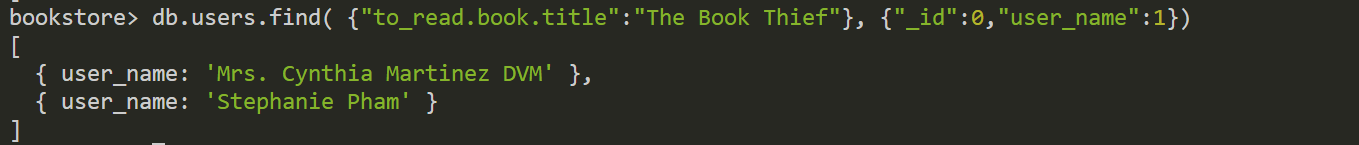
\includegraphics[width=1\textwidth]{images/MRCGAB004/1.png}
\end{center}
\subsection{2}
\label{sec:org1badb2b}
\textbf{Description}\\
test\\
\linebreak
\textbf{Query}
\begin{minted}[]{js}
sauce
\end{minted}
\linebreak
\textbf{Output}\\
\begin{center}
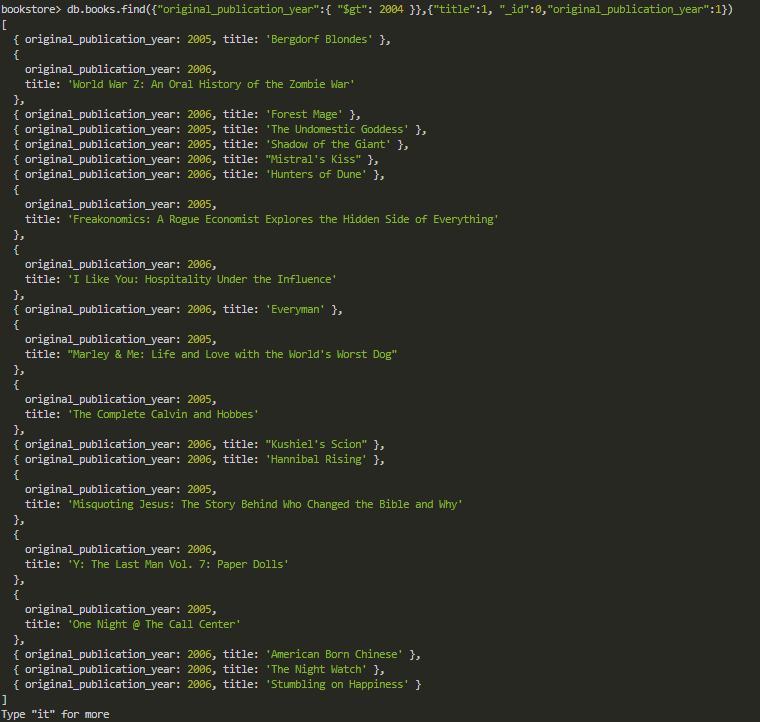
\includegraphics[width=1\textwidth]{images/MRCGAB004/2.png}
\end{center}
\subsection{3}
\label{sec:org3aaf871}
\textbf{Description}\\
test\\
\linebreak
\textbf{Query}
\begin{minted}[]{js}
sauce
\end{minted}
\linebreak
\textbf{Output}\\
\begin{center}
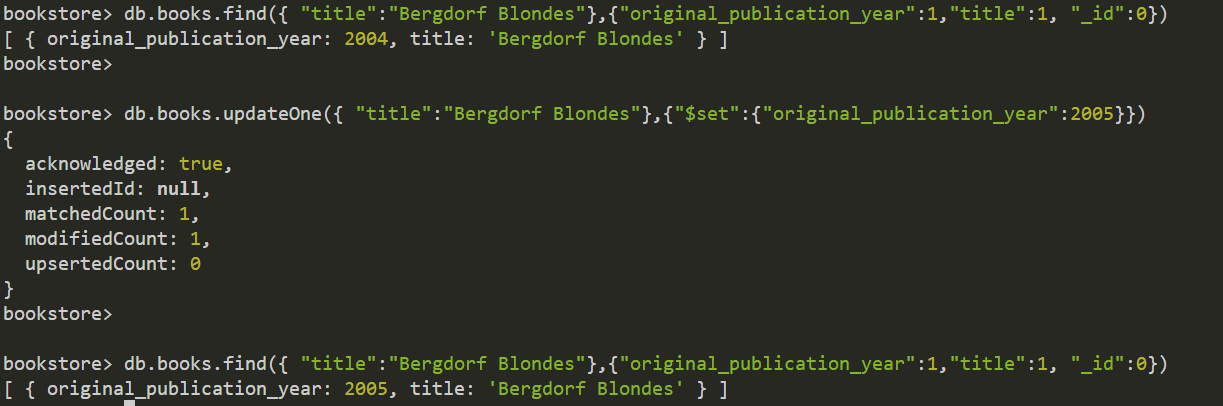
\includegraphics[width=1\textwidth]{images/MRCGAB004/3.png}
\end{center}
\subsection{4}
\label{sec:org68da79b}
\textbf{Description}\\
test\\
\linebreak
\textbf{Query}
\begin{minted}[]{js}
sauce
\end{minted}

\linebreak
\textbf{Output}\\
\begin{center}
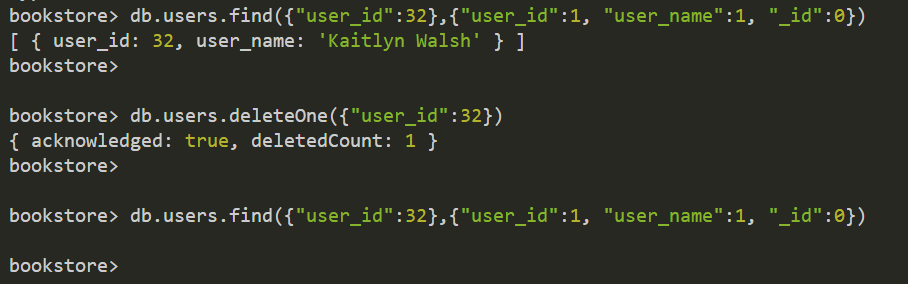
\includegraphics[width=1\textwidth]{images/MRCGAB004/4.png}
\end{center}
\end{document}
